\documentclass[tikz,border=3pt]{standalone}
\usepackage{amsmath}
\usepackage{tikz}
\usetikzlibrary{arrows.meta}
\begin{document}
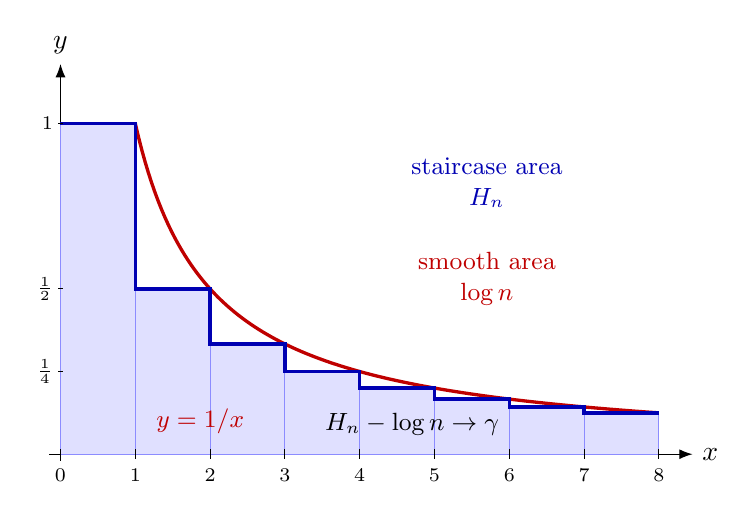
\begin{tikzpicture}[>=Latex,x=0.95cm,y=4.2cm]
  \draw[->] (-0.15,0) -- (8.45,0) node[right] {$x$};
  \draw[->] (0,-0.02) -- (0,1.18) node[above] {$y$};
  \foreach \k in {1,...,8} {
    \pgfmathsetmacro{\h}{1/\k}
    \fill[blue!12] (\k-1,0) rectangle (\k,\h);
    \draw[blue!45] (\k-1,0) rectangle (\k,\h);
  }
  \draw[red!75!black,very thick,domain=1:8,samples=160]
    plot (\x,{1/\x});
  \draw[blue!70!black,very thick]
    (0,1) -- (1,1) -- (1,0.5) -- (2,0.5) -- (2,0.3333) -- (3,0.3333)
    -- (3,0.25) -- (4,0.25) -- (4,0.2) -- (5,0.2)
    -- (5,0.1667) -- (6,0.1667) -- (6,0.1429) -- (7,0.1429)
    -- (7,0.125) -- (8,0.125);
  \foreach \x in {0,1,2,...,8} {
    \draw (\x,0.015) -- (\x,-0.015) node[below,font=\scriptsize] {$\x$};
  }
  \foreach \y/\lab in {1/1,0.5/\frac12,0.25/\frac14} {
    \draw (-0.03,\y) -- (0.03,\y) node[left,font=\scriptsize] {$\lab$};
  }
  \node[align=center,font=\small,blue!70!black] at (5.7,0.82)
    {staircase area\\$H_n$};
  \node[red!75!black,font=\small,anchor=west] at (1.15,0.10) {$y=1/x$};
  \node[align=center,font=\small,red!75!black] at (5.7,0.53)
    {smooth area\\$\log n$};
  \node[align=center,font=\small] at (4.7,0.09)
    {$H_n-\log n\to\gamma$};
\end{tikzpicture}
\end{document}
